\documentclass[xcolor=dvipsnames]{beamer}
\usepackage{xmpmulti}
\usepackage{comp2402}

%\usepackage[T1]{fontenc}
%\usepackage[sfdefault,black]{merriweather} %% Option 'black' gives heavier bold face 
%
%

%\usepackage{libris}
%\renewcommand*\familydefault{\sfdefault} %% Only if the base font of the document is to be sans serif
%\usepackage[T1]{fontenc}
%
% For source code:
\usepackage{minted}
\usepackage{mdframed}
\surroundwithmdframed{minted}

% For aligning tables
\usepackage{array}

\newcommand{\mi}[1]{\multiinclude[<+>][start=1,format=pdf]{#1}}

\title{Computer Architecture Through Binary Searching}
\author{Pat Morin}
\date{Carleton University}


\begin{document}

\begin{frame}
  \titlepage
  \centerline{
    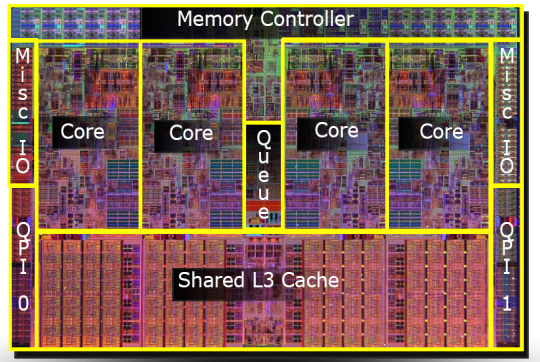
\includegraphics[height=1in]{images/nehalemdie}
    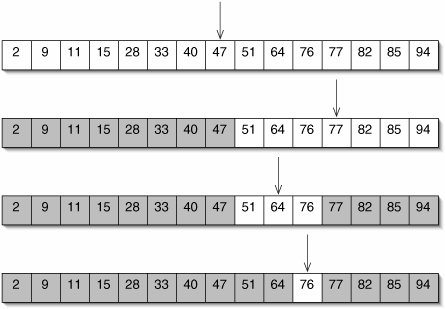
\includegraphics[height=1in]{images/binary-search}
    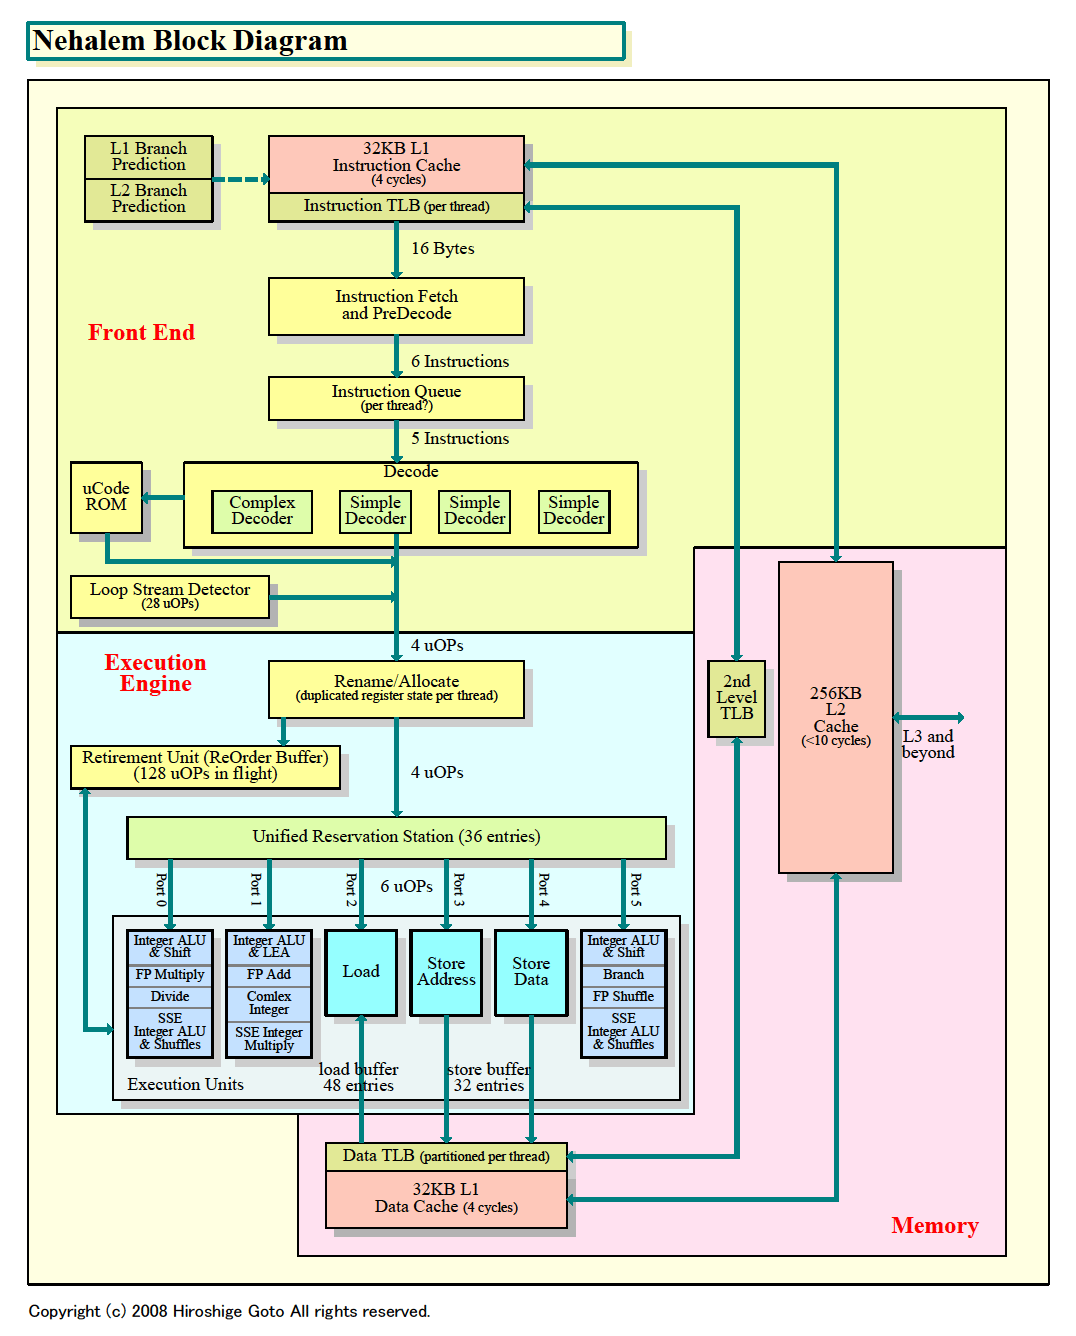
\includegraphics[height=1in]{images/nehalem-block}
  }
\end{frame}

\begin{frame}
  \frametitle{Microprocessor Architecture: Programmer's View}
  \framesubtitle{Von Neumann Architecture}

  \begin{center}
    \includegraphics[scale=0.85]{figs/programmers-view} 
  \end{center}
  
%  \begin{itemize}
%    \item<+->CPU repeatedly
%    \begin{itemize}
%      \item<+->Fetches an instruction (from RAM)
%      \item<+->Decodes the instruction
%      \item<+->Executes the instruction
%    \end{itemize}
%    \item<+->Instructions include:
%     \begin{itemize}
%      \item<+->Arithmetic operations on CPU registers
%      \item<+->Moving data between registers and RAM
%    \end{itemize}
%  \end{itemize}
  
\end{frame}


\begin{frame}
  \frametitle{Binary Search}
  \framesubtitle{The Classic Data Structure/Query Algorithm}

  \begin{center}
    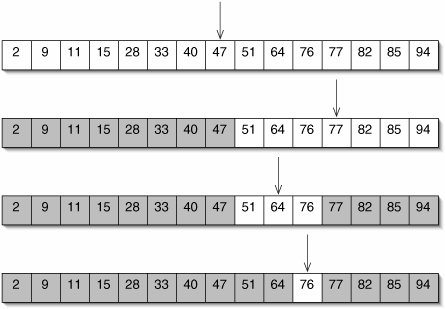
\includegraphics[width=.9\textwidth]{images/binary-search}
  \end{center}

\end{frame}


\begin{frame}[fragile]
  \frametitle{Binary Search}
  \framesubtitle{Branchy Code}

\begin{minted}{c++}
template<typename T, typename I>
I sorted_array<T,I>::branchy_search(T x) const {
    I lo = 0, hi = n;
    while (lo < hi) {
        I m = (lo + hi) / 2;
        if (x < a[m]) {
            hi = m;
        } else if (x > a[m]) {
            lo = m+1;
        } else {
            return m;
        }
    }
    return hi;
}
\end{minted}
\end{frame}

\begin{frame}[fragile]
  \frametitle{Binary Search: Analysis}

  \begin{itemize}
    \item<+->Each iteration of binary search either:
    \begin{itemize}
      \item<+->terminates (because \mintinline{c++}{x==a[m]})
      \item<+->terminates (because \mintinline{c++}{lo==hi})
      \item<+->Reduces \mintinline{c++}{hi-lo} by a factor of 2
    \end{itemize}
    \item<+->Binary search terminates after at most $\log_2 n$ iterations
    \item<+->Doubling the size of the array adds only one more iteration
  \end{itemize}
\end{frame}

\begin{frame}
  \frametitle{Binary Search: Experiments}
  \begin{center}
    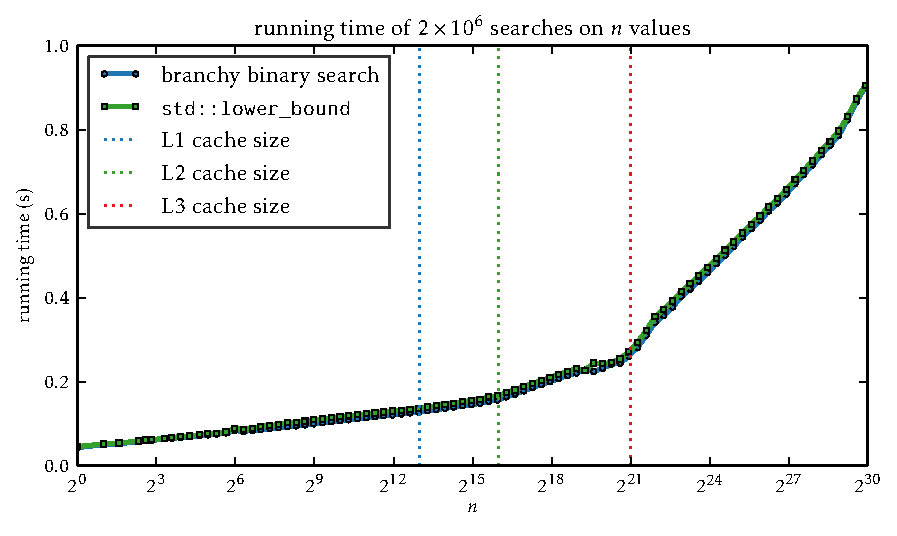
\includegraphics{graphs/sorted-i}
  \end{center}
\end{frame}

\begin{frame}[fragile]
  \frametitle{Binary Search}
  \framesubtitle{Branchy Assembly Code}

%\vspace{-2em}
\tiny
%\resizebox{\textwidth}{\textheight}{
\begin{minted}{nasm}
       .cfi_startproc
       movq    8(%rdi), %rax
       xorl    %ecx, %ecx
       movq    (%rdi), %r8
       cmpq    %rcx, %rax
       jbe     .L5                 ; quit if lo == hi
.L11:  leaq    (%rcx,%rax), %rdx   ; top of while loop
       shrq    %rdx
       movl    (%r8,%rdx,4), %edi  ; load a[m]
       cmpl    %edi, %esi          ; compare a[m] and x
       jnb    .L3                  ; jump if a[m] <= x
 .L8:  cmpq    %rdx, %rcx          ; a[m] > x, search first half
       movq    %rdx, %rax
       jnb     .L5
       addq    %rcx, %rdx          ; lo + hi
       shrq    %rdx                ; (lo + hi) / 2
       movl    (%r8,%rdx,4), %edi  ; load a[m]
       cmpl    %edi, %esi          ; compare a[m] and x
       jb      .L8                 ; jump if a[m] > x
 .L3:  cmpl    %edi, %esi          ; here a[m] <= x
       jbe     .L7                 ; quit if a[m] == x
       leaq    1(%rdx), %rcx
       cmpq    %rcx, %rax
       ja      .L11                ; back to top, if lo < hi
 .L5:  rep ret
 .L7:  movq    %rdx, %rax
       ret
       .cfi_endproc
\end{minted}
%}

\end{frame}

\begin{frame}
   \frametitle{The Instruction Pipeline}

   \begin{center}
      \mi{figs/pipeline}
   \end{center}
   \vspace{-1em}
   \begin{itemize}
     \item<3->Guess wrong and we have to flush the whole pipeline!
     \item<4->May take 20--24 cycles!
   \end{itemize}
\end{frame}

\begin{frame}[fragile]
   \frametitle{Branch-Free Binary Search}
   \framesubtitle{C++ Code}

   \begin{itemize}
       \item On random searches, branchy binary search will guess 
                wrong nearly 50\% of the time.
       \item Eliminate branching with conditional moves (\texttt{\color{blue}cmov})
   \end{itemize}
\begin{minted}{c++}
I sorted_array<T,I>::branchfree_search(T x) const {
  const T *base = a;
  I n = this->n;
  while (n > 1) {
    const I half = n / 2;
    base = (base[half] < x) ? &base[half] : base;
    n -= half;
  }
  return (*base < x) + base - a;
}
\end{minted}
\end{frame}

\begin{frame}[fragile]
   \frametitle{Branch-Free Binary Search}
   \framesubtitle{Assembly Code}

\tiny
\begin{minted}{nasm}
  .cfi_startproc
  movq    8(%rdi), %rdx       ; move n into rdx
  movq    (%rdi), %r8         ; move a into r8
  cmpq    $1, %rdx            ; compare n and 1
  movq    %r8, %rax           ; move base into rax
  jbe    .L2                  ; quit if n <= 1
.L3:
  movq    %rdx, %rcx          ; put n into rcx
  shrq    %rcx                ; rcx = half = n/2
  leaq    (%rax,%rcx,4), %rdi ; load &base[half] into rdi
  cmpl    %esi, (%rdi)        ; compare x and base[half]
  cmovb   %rdi, %rax          ; set base = &base[half] if x > base[half]
  subq    %rcx, %rdx          ; n = n - half
  cmpq    $1, %rdx            ; compare n and 1
  ja      .L3                   ; keep going if n > 1
.L2:
  cmpl    %esi, (%rax)        ; compare x to *base
  sbbq    %rdx, %rdx          ; set dx to 00..00 or 11...11
  andl    $4, %edx            ; set dx to 0 or 4 
  addq    %rdx, %rax          ; add dx to base
  subq    %r8, %rax           ; compute base - a (* 4)
  sarq    $2, %rax            ; (divide by 4)
  ret
  .cfi_endproc
\end{minted}
\end{frame}

\begin{frame}[fragile]
   \frametitle{Branch-Free Binary Search}
   \framesubtitle{Performance}

   \begin{center}
     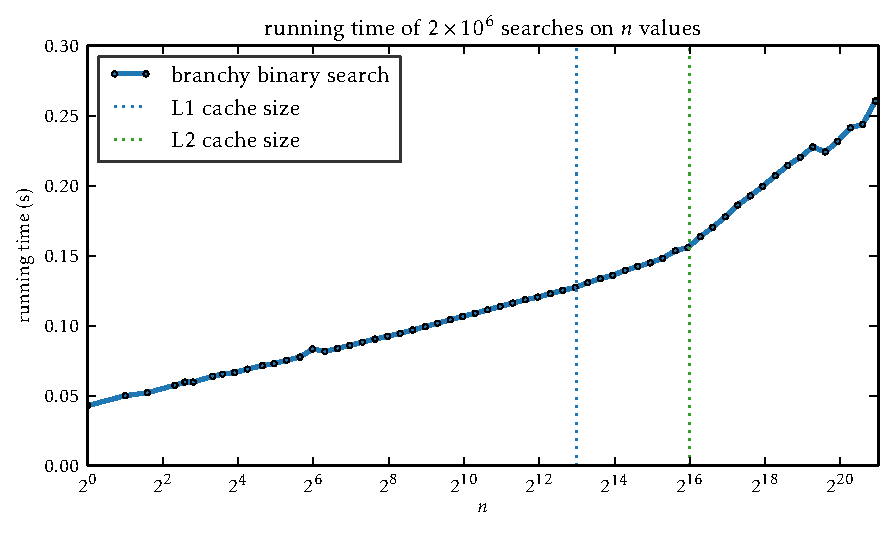
\includegraphics{graphs/sorted-ii}
   \end{center}
\end{frame}


\begin{frame}
   \frametitle{The Memory Hierarchy}

   \begin{center}
     \only<+>{\includegraphics[scale=0.85]{figs/programmers-view}}%
     \only<+->{\includegraphics[scale=0.85]{figs/caches}}
   \end{center}
   \begin{itemize}
     \item<+->Sizes: RAM (GB), L3 (MB), L2 (100's of KB), L1 (KB)
     \item<+->Speeds: RAM (100 cycles), L3 (40 cycles), L2 (10 cycles), L1 (4 cycles)
   \end{itemize}
   
\end{frame}

\begin{frame}
   \frametitle{Branch-Free Binary Search}
   \framesubtitle{Performance}

   \begin{center}
     \only<+>{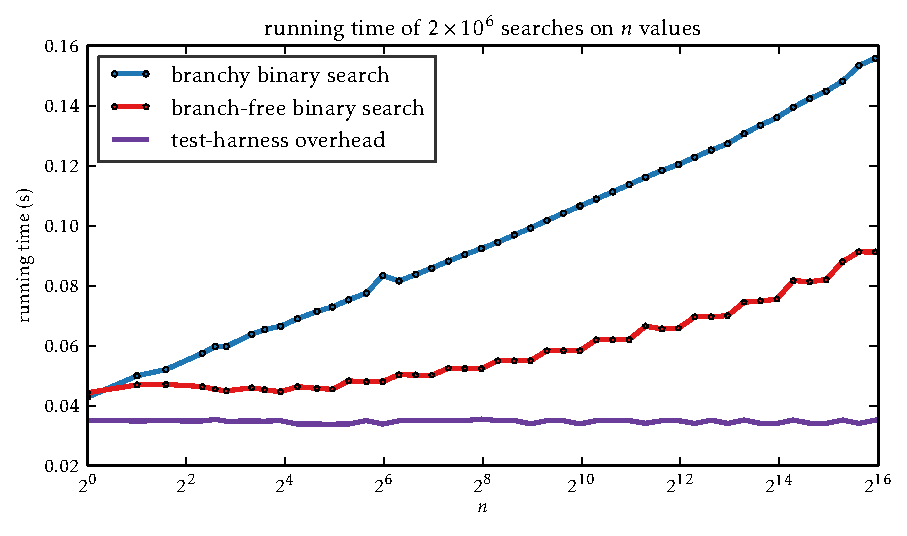
\includegraphics{graphs/sorted-iii}}%
     \only<+>{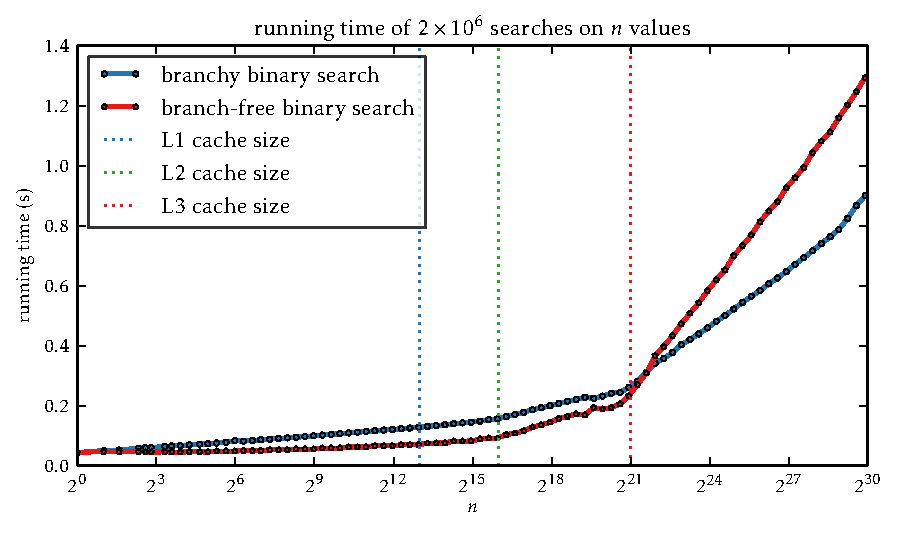
\includegraphics{graphs/sorted-iv}}%
     \only<+>{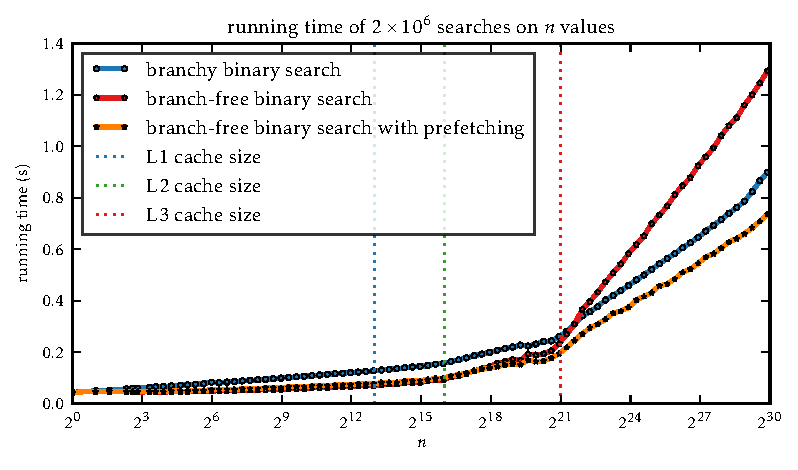
\includegraphics{graphs/sorted-v}}%
     \only<+->{\includegraphics[scale=0.85]{graphs/sorted-vi}\\[-2ex]{Wait, what?}}
   \end{center}
\end{frame}

\begin{frame}[fragile]
   \frametitle{Branchy versus Branch-Free Binary Search}
   \framesubtitle{Performance}

   \begin{tabular}{m{.48\textwidth}m{.48\textwidth}}
\tiny
 \begin{minted}{c++}
template<typename T, typename I>
I sorted_array<T,I>::branchy_search(T x) {
    I lo = 0, hi = n;
    while (lo < hi) {
        I m = (lo + hi) / 2;
        if (x < a[m]) {
            hi = m;
        } else if (x > a[m]) {
            lo = m+1;
        } else {
            return m;
        }
    }
    return hi;
}
\end{minted}
&
     \includegraphics[scale=0.5]{graphs/sorted-vi}
\end{tabular}
\begin{itemize}
  \item<+-> Branch-prediction is wrong $50\%$ the time
     \begin{itemize}
       \item<+-> Causes costly pipeline flush
     \end{itemize}
  \item<+-> Branch-prediction is right $50\%$ the time
      \begin{itemize}
       \item<+-> Puts memory subsystem to work loading from memory
     \end{itemize}
  \item<+->RAM latency $\approx100$ cycles, pipeline latency $\approx 20$ cycles
\end{itemize}
\end{frame}

\begin{frame}[fragile]
   \frametitle{Branch-Free Binary Search with Prefetching}
   \framesubtitle{The best of both worlds}

   {\tiny
   \begin{minted}{c++}
template<typename T, typename I>
I sorted_array<T,I>::_branchfree_search(T x) const {
    const T *base = a;
    I n = this->n;
    while (n > 1) {
        I half = n / 2;
        __builtin_prefetch(base + half/2, 0, 0);
        __builtin_prefetch(base + half + half/2, 0, 0);
        base = (base[half] < x) ? base+half : base;
        n -= half;
    }
    return (*base < x) + base - a;
}
   \end{minted}
   }
   \includegraphics[width=.5\textwidth]{graphs/sorted-vii}
   \includegraphics[width=.5\textwidth]{graphs/sorted-viii}

\end{frame}

\begin{frame}[fragile]
   \frametitle{The Story So Far}

   \begin{itemize}
      \item<+->Long processor pipelines require branch prediction
               for performance
      \begin{itemize}
         \item<+->Branch mispredictions are expensive (20-25 cycles)
         \item<+->Branches can sometimes be avoided using 
                  \mintinline{nasm}{cmov}
      \end{itemize}
      \item<+->Memory is a hierarchy
      \begin{itemize}
         \item<+->L1, L2, L3, RAM\only<+->{, Disk}\only<+->{, Cloud}%
            \only<+->{,\ldots}
         \item<+->Memory subsystem \emph{prefetches} as soon as it can
         \item<+->We can prefetch explicitly
      \end{itemize}
      \item<+->Long pipelines and memory hierarchy interact in surprising
               ways
   \end{itemize}
\end{frame}

\begin{frame}
   \frametitle{Cache Lines}

   \begin{itemize}
      \item<+-> RAM and caches are organized into \emph{lines}
      \begin{itemize}
        \item<+-> 64 bytes wide
      \end{itemize}
      \item<+-> Accessing a single word of RAM loads an entire line
         into the cache hierarchy ($B$ items)
   \end{itemize}
   \begin{center}
      \only<1-2>{\includegraphics{figs/cache-lines-1}}%
      \only<3->{\includegraphics{figs/cache-lines-2}}
   \end{center}
   \begin{itemize}
        \item<+->Accessing a single item costs as much as accessing a whole cache line
   \end{itemize}
\end{frame}

\begin{frame}
   \frametitle{Binary Search is Bad for Locality}
   \framesubtitle{Actually, sorted order is bad}

   \begin{itemize}
      \item<+->Binary search loads a lot of data that it never looks at
   \end{itemize}
   \begin{center}
      \mi{figs/binary-search-bad}%
   \end{center}
   \begin{itemize}
      \item<11->Loads $\log n - \log B$ cache lines
      \item<12->Example: $n =2^{30}$, $B=16$, so $\log n - \log B=26$
   \end{itemize}
\end{frame}


\begin{frame}
   \frametitle{B-Trees}

   \begin{itemize}
      \item<+->Use a $(B+1)$-ary search tree
      \item<+->Stores $B$ items per node (node fits neatly into cache line)
   \end{itemize}
   \begin{center}
      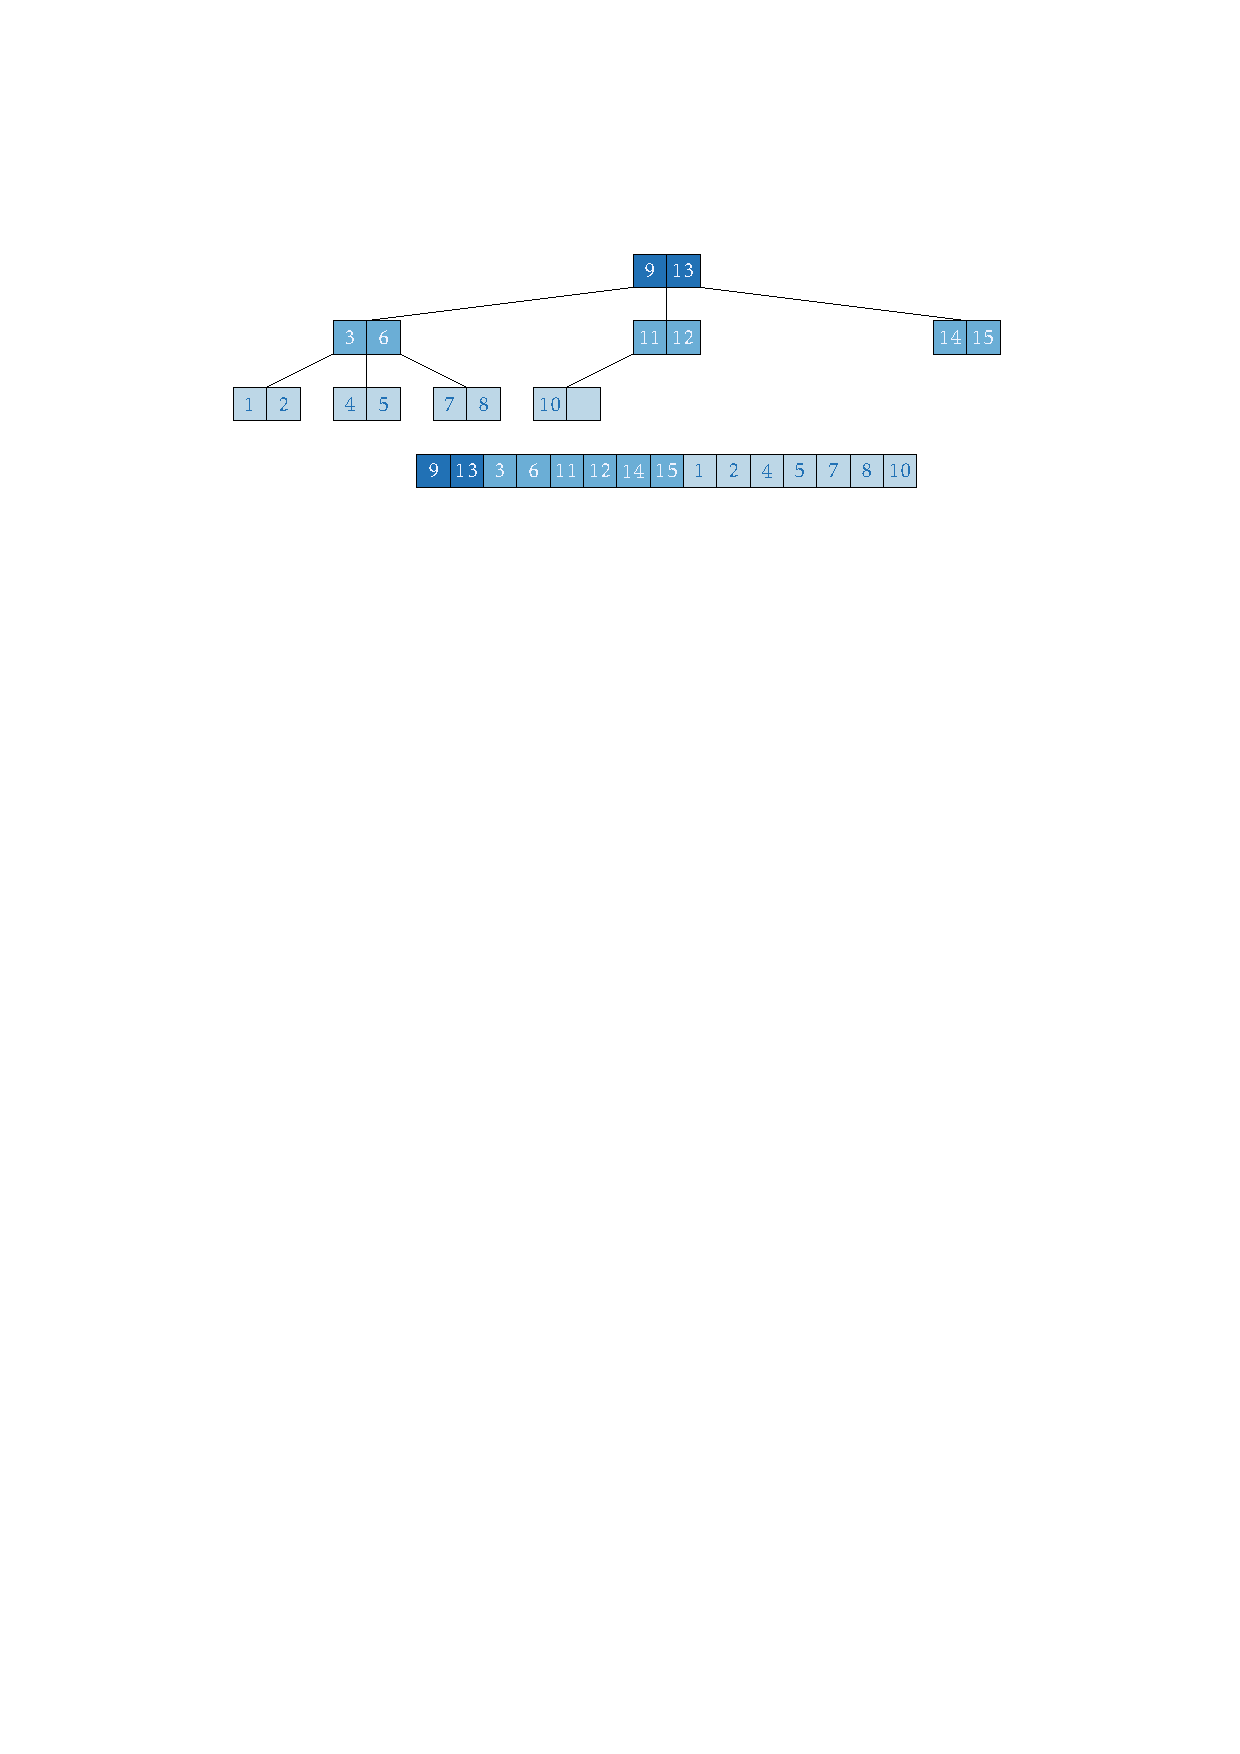
\includegraphics[width=.98\textwidth]{figs/btree}
   \end{center}
   \begin{itemize}
      \item<+->Lay nodes out into an array
   \end{itemize}
\end{frame}
 

\begin{frame}
   \frametitle{B-Tree Search}

   \begin{center}
      \mi{figs/btree-search}
   \end{center}
   \begin{itemize}
      \item<13->Accesses $\lceil\log_{B+1} n\rceil=\left\lceil\frac{\log n}{\log(B+1)}\right\rceil$ cache lines
      \item<14->Does binary search within each cache line: $\lceil\log(B+1)\rceil$ comparisons
      \item<15->Example: $n=2^{30}$, $B=16$, $\lceil\log_{B+1} n\rceil = 8$
      \item<16->Compared to 26 cache lines with binary search
   \end{itemize}
\end{frame}

\begin{frame}
   \frametitle{B-Tree Search}
   \framesubtitle{Performance}
 
   \begin{center}
      \only<1>{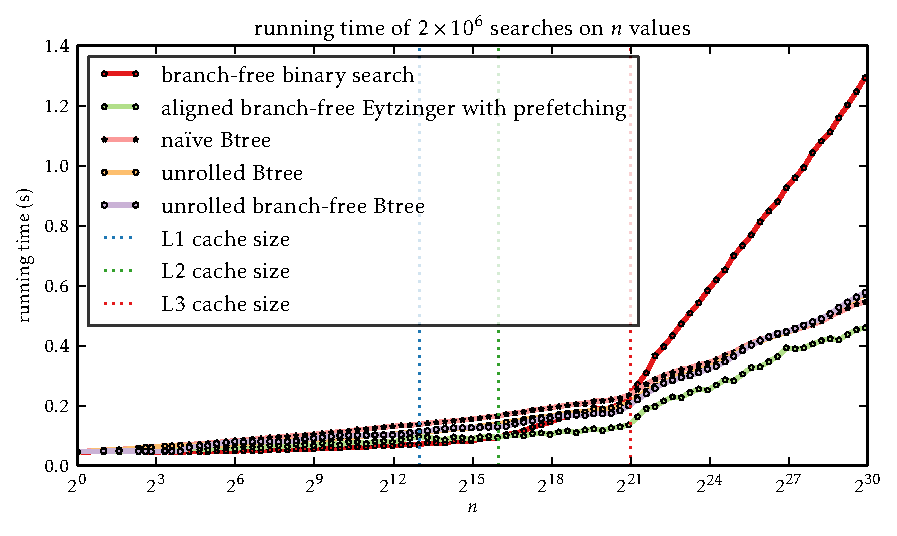
\includegraphics[height=.6\textheight]{graphs/btree-i} \\ Good!}
      \only<2>{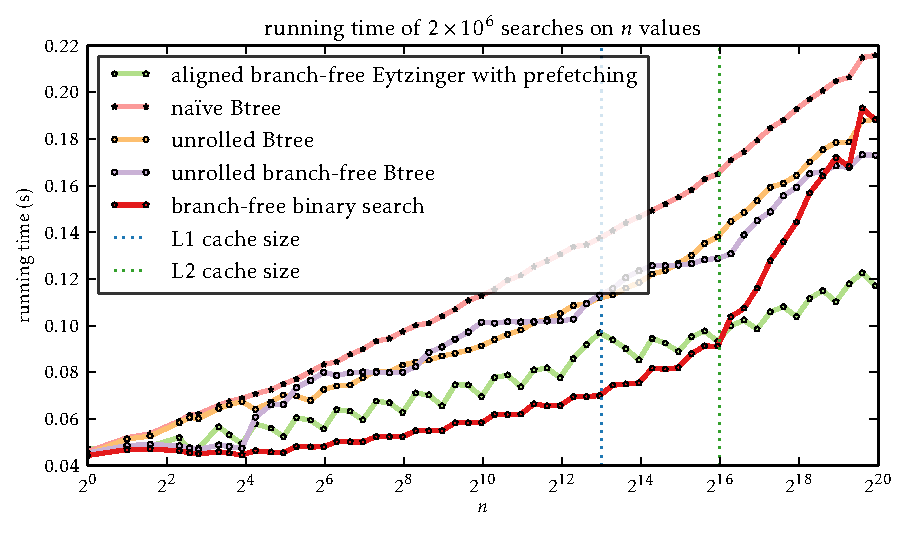
\includegraphics[height=.6\textheight]{graphs/btree-ii} \\ Bad!}
   \end{center}
\end{frame}

\begin{frame}
   \frametitle{B-Tree Search Problems}
   \framesubtitle{Why are B-Trees so slow?}
    
   \begin{itemize}
      \item<+->Internal binary search has $B+1$ possible outcomes:
      \begin{itemize}
        \item<+->Example: $B=16$, 
                  $\lceil\log(B+1)\rceil = \lceil 4.08\rceil = 5$
      \end{itemize}
      \item<+->Big increase in search time for each new level 
      \begin{itemize}
        \item<+->Example: $n=2^{10}$, $B=16$, 
                  $\lceil\log_{B+1}n\rceil = \lceil 2.44\rceil = 3$
        \item<+->$3\times 5 = 15$ comparisons (versus 11 for binary search)
      \end{itemize}
   \end{itemize}
   \begin{center}
      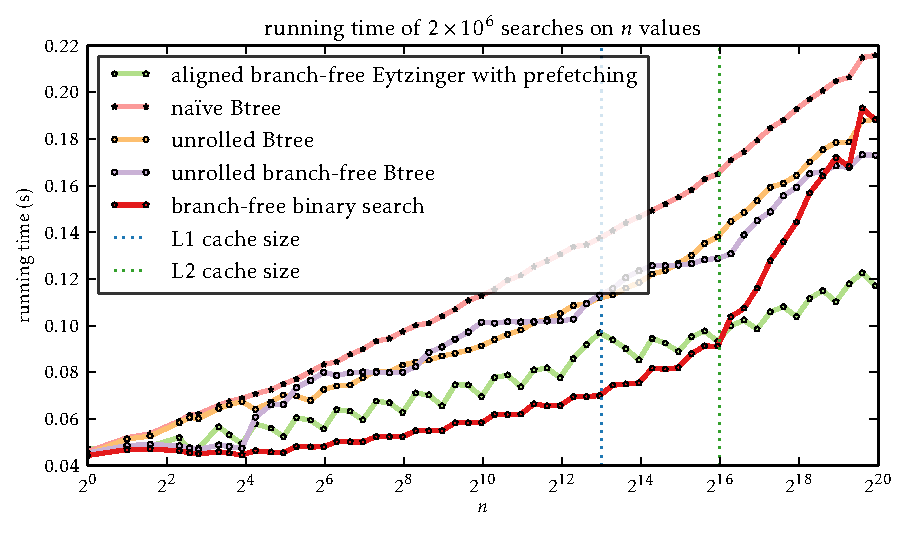
\includegraphics[height=.6\textheight]{graphs/btree-ii}
   \end{center}
\end{frame}

\begin{frame}
   \frametitle{Beating B-Trees}

   Things we know:
   \begin{enumerate}[<+->]
      \item Branch misprediction is costly
      \item Memory is chunked into 64 byte cache lines
      \item Memory subsystem can prefetch at the same time we compute
      \item B-Tree problem: When $B$ is a power of 2, $B+1$ is not
   \end{enumerate}
   \begin{itemize}
      \item<+->B-Trees take advantage of 1 \& 2.
      \item<+->B-Trees don't take advantage of 3.
      \item<+->4 is not true if we take $B=1$.
   \end{itemize}

\end{frame}

\end{document}

